\documentclass{beamer}
 
\usepackage[utf8]{inputenc}
\usepackage{mystyle}
\usepackage{diagbox}
\usepackage{subcaption}
\usepackage{tikz}

\usepgfmodule{shapes}
\usepgfmodule{plot}
\usetikzlibrary{decorations}
\usetikzlibrary{arrows}
\usetikzlibrary{shadows}  
\usetikzlibrary{snakes} 
\usetikzlibrary{shapes}
\usetikzlibrary{matrix} 
\usetikzlibrary{positioning} 
\usetikzlibrary{backgrounds}
 

\newcommand{\LSE}{\textrm{LSE}}

%Information to be included in the title page:
\title{Kernel Belief Propagation}

\begin{document}
 
\frame{\titlepage}
 
\begin{frame}
\frametitle{Motivation}
\begin{itemize}
\item Difficult to derive belief propagation messages for continuous RVs
    with complex densities, which typically rely on easy to compute conditionals
    (ie conjugacy or discrete)
\vspace{1em}
\item Instead, rewrite messages using \textbf{nonparametric} representations
of densities, i.e. sums of points in some space with no explicit parameters
\vspace{1em}
\item Approach extends to any domain on which kernels can be defined,
such as strings and graphs
\end{itemize}
\end{frame}

\begin{frame}
\frametitle{Differences from Performer-style Inference}
\begin{itemize}
\item Goal is to do approximate nonparametric inference
\item Performer speedup comes from exact inference in a smaller space
\end{itemize}
\end{frame}

\begin{frame}
\frametitle{Learning in Markov Random Fields}
\begin{itemize}
\item Pairwise MRF (typically parameterize log potentials)
$$\mathbb{P}(X) \propto \prod_{s,t \in \mcE} \Psi_{st}(X_s, X_t) \prod_{s\in\mcV} \Psi(X_s).$$
\item Estimate gradients wrt log potentials by computing edge and node marginals
via inference, ie the beliefs $\mathbb{B}(X_s, X_t)$ and $\mathbb{B}(X_s)$
\vspace{2em}
\item Belief propagation is an algorithm for performing inference
\end{itemize}
\end{frame}

\begin{frame}
\frametitle{Belief Prop (BP)}
\begin{itemize}
\item BP propagates messages from nodes to neighbours iteratively until convergence
\item Messages from $t$ to $s$
$$m_{ts}(X_s) = \int_{X_t\in\mcX} \Psi_{st}(X_s, X_t) \Psi_t(X_t)
    \prod_{u\in\delta(t)\setminus\set{s}} m_{ut}(X_t)dX_t$$
\item Belief at $s$
$$\mathbb{B}(X_s) = \Psi_s(X_s)\prod_{t\in\delta(s)} m_{ts}^*(X_s),$$
with fixed point messages $m^*$
\end{itemize}
\end{frame}

\begin{frame}
\frametitle{BP}
\begin{itemize}
\item The integrals in the messages may be difficult to compute
\vspace{2em}
\item Solution: Rewrite messages as an expectation, then approximate conditional
\begin{align*}
m_{ts}(X_s) &= \int_\mcX \mathbb{P}^*(X_t \mid X_s)
\prod_{u \in \delta(t)\setminus\set{s}} m_{ut}(X_t)dX_t\\
&= \mathbb{E}_{Xt \mid X_s}\left[
\prod_{u \in \delta(t)\setminus\set{s}} m_{ut}(X_t)\right]
\end{align*}
\item Requires fully observed model, otherwise stuck with original integral
\end{itemize}
\end{frame}

\begin{frame}
\frametitle{Nonparametric BP Baselines}
\begin{itemize}
\item Nonparametric BP requires a 2-step process of estimating conditional $\mathbb{P}^*(X_t \mid X_s)$,
    then computing messages
\vspace{2em}
\item NPBP baselines are Gaussian Mixture BP (Sudderth et al, 2003) and 
Particle BP (Ihler and McAllester, 2009)
\vspace{2em}
\item Kernel BP reduces this to a single step of matrix-vector products
\end{itemize}
\end{frame}

\begin{frame}
\frametitle{High Level Overview of Kernel Belief Propagation}
\begin{itemize}
\item Embed messages in RKHS
\vspace{2em}
\item Approximate expectations via observed samples 
\vspace{2em}
\item Compute messages with inner products
\end{itemize}
\end{frame}

\begin{frame}
\frametitle{Kernel Mean Embedding}
%% schematic summarization
\begin{figure}[t!]
  \centering
  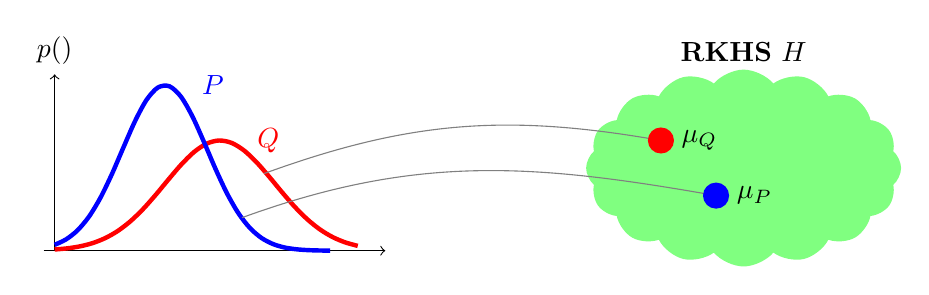
\begin{tikzpicture}[domain=0:6,scale=0.7]
      % set up locations
      \coordinate (P1) at (3.4,1.6);
      \coordinate (Q1) at (3.8,2.4);
      \coordinate (P2) at (12,2);
      \coordinate (Q2) at (11,3);

      \draw[->] (-0.2,1) -- (6,1) node[right] {$\ensuremath{\bx}$};
      \draw[->] (0,1) -- (0,4.2) node[above] {$p(\bx)$};
      \draw[color=red,smooth,domain=0:5.5,ultra thick] plot (\x,{1+2*exp(-(\x-3)*(\x-3)*0.5/1)});
      \draw[color=blue,smooth,domain=0:5,ultra thick] plot (\x,{1+3*exp(-(\x-2)*(\x-2)*0.5/0.6)});

      % the rkhs
      \node [cloud, fill=green!50, cloud puffs=16, cloud puff arc= 100,
      minimum width=4cm, minimum height=2.5cm, aspect=1] at (12.5,2.5) {};
      \node [] at (12.5,4.6) {\textbf{RKHS} $\mathscr{H}$};

      % draw the embedding
      \draw[color=gray] (P1) to[out=20,in=170] (P2);
      \draw[color=gray] (Q1) to[out=20,in=170] (Q2);

      \node [fill=blue,circle,thick,minimum width=0.1cm] at (P2) {};
      \node [right] at (12.2,2) {$\mu_{\mathbb{P}}$};
      \node [fill=red,circle,thick,,minimum width=0.1cm] at (Q2) {};
      \node [right] at (11.2,3) {$\mu_{\mathbb{Q}}$};

      \node [right] at (2.5,4) {$\color{blue} \mathbb{P}$};
      \node [right] at (3.5,3) {$\color{red} \mathbb{Q}$};
  \end{tikzpicture}
  %\caption{Embedding of marginal distributions: Each distribution is mapped into a reproducing
   % kernel Hilbert space via an expectation operation.}
  \label{fig:kme-summary}
\end{figure}

\begin{itemize}
\item Kernel mean embeddings map distributions into Hilbert spaces
\item Can approximate embedding in RKHS via sampling
\end{itemize}

\end{frame}

\begin{comment}
\frametitle{}
%% from data points to probability measures
\begin{figure}[t!]
  \centering
  \begin{subfigure}[b]{0.32\textwidth}
    \includegraphics[width=\textwidth]{survey/points.eps}
    \caption{$\bx \mapsto k(\bx,\cdot)$}
    \label{subfig:data-point}
  \end{subfigure}
  \hfill
  \begin{subfigure}[b]{0.33\textwidth}
      \includegraphics[width=\textwidth]{survey/dirac.eps}
      \caption{$\delta_{\bx} \mapsto \int k(\by,\cdot) d\delta_{\bx}(\by)$}
      \label{subfig:dirac-measure}
  \end{subfigure}
  \hfill
  \begin{subfigure}[b]{0.33\textwidth}
    \includegraphics[width=\textwidth]{survey/measure.eps}
    \caption{$\mathbb{P} \mapsto \int k(\bx,\cdot) d\mathbb{P}(\bx)$}
    \label{subfig:prob-measure}
  \end{subfigure}
  \caption{From data points to probability measures: (\subref{subfig:data-point}) An illustration of a  typical application of the kernel as a high-dimensional feature map of an individual data point. (\subref{subfig:dirac-measure}) A measure-theoretic view of high-dimensional feature map. An embedding of data point into a high-dimensional feature space can be equivalently viewed as an embedding of a Dirac measure assigning the mass 1 to each data point. (\subref{subfig:prob-measure}) Generalizing the Dirac measure point of view, we can generally extend the concept of a high-dimensional feature map to the class of probability measures.}
  \label{fig:from-point-to-measure}
\end{figure}

\end{comment}

\begin{frame}
\frametitle{Conditional Distribution Embedding}
\begin{figure}[t!]
\centering
  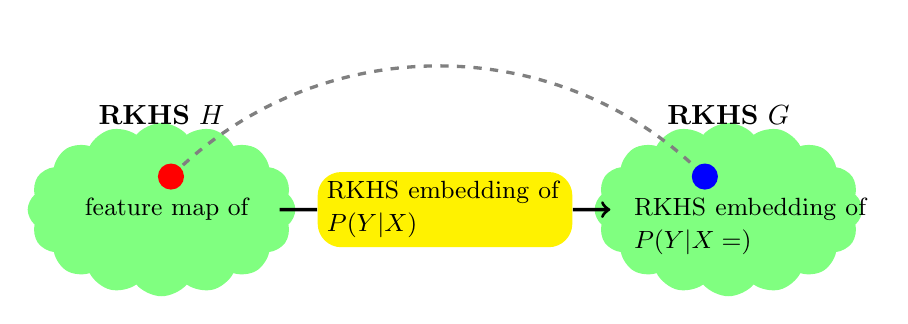
\begin{tikzpicture}[scale=0.6]
      %\draw[->] (-0.2,0.5) -- (7.5,0.5) node[right] {$X$};
      %\draw[->] (0,0.5) -- (0,3.7) node[left,yshift=-10] {$Y$};
      %\draw[rotate=-90,color=blue!10,smooth,domain=-3.5:-0.5,ultra thick] plot (\x,{1+exp(-(3+\x)*(3+\x)*0.5/0.2)});
      %\draw[rotate=-90,color=blue!15,smooth,domain=-3.5:-0.5,ultra thick] plot (\x,{1.6+exp(-(2.8+\x)*(2.8+\x)*0.5/0.3)});
      %\draw[rotate=-90,color=blue!20,smooth,domain=-3.5:-0.5,ultra thick] plot (\x,{2.2+exp(-(2.6+\x)*(2.6+\x)*0.5/0.3)});
      %\draw[rotate=-90,color=blue!25,smooth,domain=-3.5:-0.5,ultra thick] plot (\x,{2.8+exp(-(2.4+\x)*(2.4+\x)*0.5/0.3)});
      %\draw[rotate=-90,color=blue!30,smooth,domain=-3.5:-0.5,ultra thick] plot (\x,{3.4+exp(-(2.2+\x)*(2.2+\x)*0.5/0.3)});
      %\draw[rotate=-90,color=blue!35,smooth,domain=-3.5:-0.5,ultra thick] plot (\x,{4+exp(-(2.4+\x)*(2.4+\x)*0.5/0.3)});
      %\draw[rotate=-90,color=blue!40,smooth,domain=-3.5:-0.5,ultra thick] plot (\x,{4.6+exp(-(2.5+\x)*(2.5+\x)*0.5/0.5)});
      %\draw[rotate=-90,color=blue!45,smooth,domain=-3.5:-0.5,ultra thick] plot (\x,{5.2+exp(-(2.6+\x)*(2.6+\x)*0.5/0.5)});
      %\draw[rotate=-90,color=blue!50,smooth,domain=-3.5:-0.5,ultra thick] plot (\x,{5.8+exp(-(2.9+\x)*(2.9+\x)*0.5/0.6)});
      %\node [rotate=-90] at (0.6,2.6) {$P(Y|X=x)$};
      %\node [rotate=-90] at (4,4.5) {$P(Y|X)$};
      %\node [rotate=-90] at (0.6,2.6) {$\mathbb{P}(Y|X)$};

      %%%%%%

      % set up locations
      \coordinate (P1) at (-2.3,5.7);
      \coordinate (P2) at (9,5.7);

      %\draw[->] (-0.2,1) -- (6,1) node[right] {$x$};
      %\draw[->] (0,1) -- (0,4.2) node[above] {$p(x)$};
      %\draw[color=red,smooth,domain=0:5.5,ultra thick] plot (\x,{1+2*exp(-(\x-3)*(\x-3)*0.5/1)});
      %\draw[color=blue,smooth,domain=0:5,ultra thick] plot (\x,{1+3*exp(-(\x-2)*(\x-2)*0.5/0.6)});

      %%%%%%

      % the rkhs of X
      \node [cloud, fill=green!50, cloud puffs=16, cloud puff arc= 100,
      minimum width=3.4cm, minimum height=2.2cm, aspect=1] at (-2.5,5) {};
      \node [] at (-2.5,7) {\textbf{RKHS} $\mathscr{H}$};

      % the rkhs of Y
      \node [cloud, fill=green!50, cloud puffs=16, cloud puff arc= 100,
      minimum width=3.4cm, minimum height=2.2cm, aspect=1] at (9.5,5) {};
      \node [] at (9.5,7) {\textbf{RKHS} $\mathscr{G}$};

      %%%%%%%
      % draw the embedding
      %\node(n1){n1};
      %\node(n2)[below right=3cm and 3cm of n1]{n2};
      % \node [text width = 4cm] at (3.5,8) {};
      %\draw[->] (P1)--(text2)--(n2) node[right] {};
      %\draw[->] (0,5)--(text)--(7,5) node[right] {};
      \draw[->,color=gray,dashed,very thick] (P1) to[out=45,in=135] (P2);

      \node [fill=blue,circle,minimum width=0.05cm] at (P2) {};
      \node [below,yshift=-0.15cm,xshift=0.6cm, text width=3cm] at (P2) {{\small RKHS embedding of $\mathbb{P}(Y|X=\bx)$}};
      \node [fill=red,circle,minimum width=0.05cm] at (P1) {};
      \node [below,yshift=-0.15cm] at (P1) {{\small feature map of $\bx$}};

      \coordinate (n1) at (0,5);
      \coordinate (n2) at (7,5);
      %\node(n1){n1};
      %\node(n2)[below right=3cm and 3cm of n1]{n2};
      \path (n1) -- node[sloped, fill=yellow, rounded corners=.3cm, text width=3cm] (text) {{\small RKHS embedding of $\mathbb{P}(Y|X)$}} (n2);
      \draw[->, very thick] (n1)--(text)--(n2) node[right] {};
      %\draw[->] (0,5)--(text)--(7,5) node[right] {};

      %%%%%%%

      %\draw[->] (-0.2,9) -- (4,9) node[right] {$\by$};
      %\draw[->] (0,9) -- (0,11.2) node[above] {$p(\by|\bx)$};
      %\draw[color=red,smooth,domain=0:4,ultra thick] plot (\x,{9.2+1.8*exp(-(\x-2)*(\x-2)*0.5/0.3)});
      %\node [right] at (3,10) {$\mathbb{P}(Y|X=\x)$};
    \end{tikzpicture}
  %\caption{From marginal distribution to conditional distribution: unlike the embeddings shown in Figure \ref{fig:marginal-embedding}, the embedding of 
  %conditional distribution $\mathbb{P}(Y|X)$ is not a single element in the RKHS. Instead, it may be viewed as a family of Hilbert space embeddings of conditional distributions $\pp{P}(Y|X=\x)$ indexed by the conditioning variable $X$. In other words, the conditional mean embedding can be viewed as an operator from $\hbspace$ to $\hbspg$(cf. \S\ref{sec:regression-view}).}
  \label{fig:conditional-embedding-summary}
\end{figure}

\begin{itemize}
\item Embed conditional probability function as an operator
\end{itemize}

\end{frame}

\begin{frame}
\frametitle{Why the focus on nonparametric?}
\begin{itemize}
\item The sell is that this works as an approximation for inference in models
    where the messages are difficult to derive, i.e. complex distributions
\vspace{2em}
\item Kernel mean embeddings also apply to messages that are easy to derive,
    but we may want to approximate for computational benefits
\end{itemize}
\end{frame}

\begin{frame}
\frametitle{Definitions}
\begin{itemize}
\item Domain $\mcX$
\vspace{1em}
\item Hilbert space $\mathscr{H}$ of functions on $\mcX\mapsto\R$
    with inner product $\langle\cdot,\cdot\rangle$, kernel $K$,
    and feature map $\phi$
\vspace{1em}
\item The point evaluation property, 
ie that function evaluation is an inner product,
$$\langle f, K(x, \cdot) \rangle = f(x),$$
implies the reproducing property:
$$ \langle K(x,\cdot), K(y, \cdot) \rangle = K(x,y) = \langle \phi(x), \phi(y) \rangle$$
\end{itemize}
\end{frame}

\begin{frame}
\frametitle{Why is reproducing property needed}
\begin{itemize}
\item ???
\end{itemize}
\end{frame}

\begin{frame}
\frametitle{Theorem Notes}
\begin{itemize}
\item Riesz representation theorem: If operator $\mcA: \mathscr{H} \to \R$
is bounded, then there exists a representer $g_\mcA \in \mathscr{H}$ st
$$A[f] = \langle f, g_\mcA \rangle, \forall f \in \mathscr{H}.$$
\item Point evaluation property: In an RKHS, consider the evaluation functional
$\mcF_\bx(f) = f(\bx)$. Riesz representation theorem tells us there exists a
representer $k_\bx: \mathscr{H}\to\R$ st
$$\mcF_\bx(f) = \langle f, k_\bx\rangle = f(\bx),$$
referred to as the reproducing kernel for the point $\bx$.
\item The reproducing property is a special case of the point evaluation
property. Consider the kernel $k: \mcX \times \mcX \to \R$,
and define $f(\bx) = k(\by, \bx)$ for all $\by \in \mcX$.
Applying the point evaluation property yields
$$f(\bx) = \langle k(\bx, \cdot),  k(\by, \cdot)\rangle,$$
where $k(\bx, \cdot)$ is the canonical feature map denoted by $\phi: \mcX\to\mathscr{H}$.
\item Alternatively you can start by assuming the kernel is positive definite ()
\end{itemize}
\end{frame}

\begin{frame}
\frametitle{Refs}
\bibliography{references}
\end{frame}

\end{document}
